\chapter{系统配置}

\begin{quotation}
滚滚长江东逝水,浪花淘尽英雄。是非成败转头空。青山依旧在,几度夕阳红。

白发渔樵江渚上,惯看秋月春风。一壶浊酒喜相逢。古今多少事,都付笑谈中。
\begin{flushright}
---~杨慎《临江仙》
\end{flushright}
\end{quotation}

\section{helloworld}
直接上代码
\begin{code}
int fun1(int a, int b)
{
    int c;
    c = 10;
    return 0;
}
int main(int argc, char *argv[])
{
    int a;
    a = fun1(1, 2);
    return 0;
}
\end{code}
保存上述代码为helloworld\_c.c

\section{build}
编译代码并且拷贝到nfs中,以使arm板子能运行改程序
\begin{code}
arm-linux-gcc -g helloworld_c.c -o helloworld_c.arm
cp helloworld_c.arm destdir
\end{code}

\section{run}
使用gdbserver运行代码,客户端(PC)进行远程调试
arm板运行如下命令
\begin{code}
echo 0 > /proc/sys/kernel/randomize_va_space "调整每次程序启动为同一个栈起始地址,方便调试
gdbserver yourBoardIPAddress:888 helloworld_c.arm
\end{code}
pc运行如下命令
\begin{code}
vim helloworld_c.c "打开文件
F7 "映射vimgdb快捷键
file helloworld_c.arm "加载helloworld_c.arm文件符号
target remote yourBoardIPAddress:888 "开始远程调试
Ctrl+b "在helloworld_c.c下断点
Shift+c "continue运行
ni "进入汇编调试模式
si "汇编过程调用单步进入
\end{code}

\section{ASM}
\begin{code}
Dump of assembler code for function main:
0x00008454 <main+0>:	mov	r12, sp
0x00008458 <main+4>:	stmdb	sp!, {r11, r12, lr, pc}
0x0000845c <main+8>:	sub	r11, r12, #4	; 0x4
0x00008460 <main+12>:	sub	sp, sp, #12	; 0xc
0x00008464 <main+16>:	str	r0, [r11, #-16]
0x00008468 <main+20>:	str	r1, [r11, #-20]
0x0000846c <main+24>:	mov	r0, #1	; 0x1
0x00008470 <main+28>:	mov	r1, #2	; 0x2
0x00008474 <main+32>:	bl	0x8428 <fun1>
0x00008478 <main+36>:	str	r0, [r11, #-24]
0x0000847c <main+40>:	mov	r0, #0	; 0x0
0x00008480 <main+44>:	sub	sp, r11, #12	; 0xc
0x00008484 <main+48>:	ldmia	sp, {r11, sp, pc}
End of assembler dump.

Dump of assembler code for function fun1:
0x00008428 <fun1+0>:	mov	r12, sp
0x0000842c <fun1+4>:	stmdb	sp!, {r11, r12, lr, pc}
0x00008430 <fun1+8>:	sub	r11, r12, #4	; 0x4
0x00008434 <fun1+12>:	sub	sp, sp, #12	; 0xc
0x00008438 <fun1+16>:	str	r0, [r11, #-16]
0x0000843c <fun1+20>:	str	r1, [r11, #-20]
0x00008440 <fun1+24>:	mov	r3, #10	; 0xa
0x00008444 <fun1+28>:	str	r3, [r11, #-24]
0x00008448 <fun1+32>:	mov	r0, #0	; 0x0
0x0000844c <fun1+36>:	sub	sp, r11, #12	; 0xc
0x00008450 <fun1+40>:	ldmia	sp, {r11, sp, pc}
End of assembler dump.
\end{code}

\section{分析}
本文从代码段0x0000846c开始讲解
每张图都是在还没有执行该指令时读取并绘制的

\begin{figure}[htbp]%位置选项
\centering
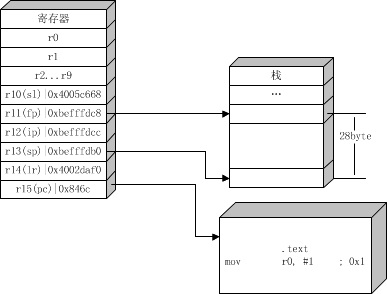
\includegraphics[bb=0 0 387 294,scale=0.7]{armapcs1_1.png}
\caption{准备压入func1参数的a}
\label{fig:anna}
\end{figure}

\begin{figure}[htbp]%位置选项
\centering
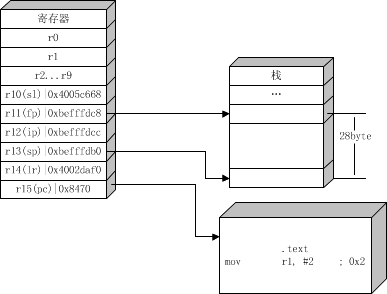
\includegraphics[bb=0 0 387 294,scale=0.7]{armapcs1_2.png}
\caption{已经压入func1参数的a 准备压入func1参数的b}
\label{fig:anna}
\end{figure}

\begin{figure}[htbp]%位置选项
\centering
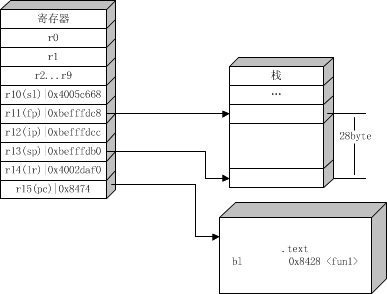
\includegraphics[bb=0 0 387 294,scale=0.7]{armapcs1_3.png}
\caption{已经压入func1参数的b 准备调用func1}
\label{fig:anna}
\end{figure}

\begin{figure}[htbp]%位置选项
\centering
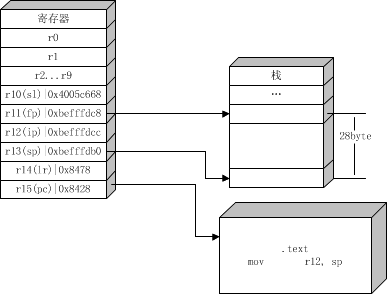
\includegraphics[bb=0 0 387 294,scale=0.7]{armapcs1_4.png}
\caption{转到func1代码段执行 准备将当前栈顶指针暂存入r12(ip),方便计算当前func1的fp指针}
\label{fig:anna}
\end{figure}

\begin{figure}[htbp]%位置选项
\centering
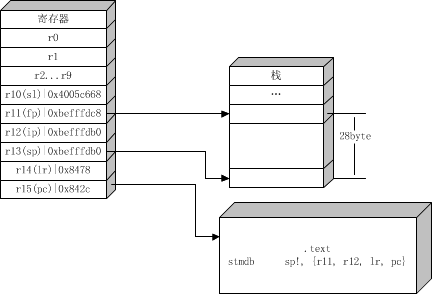
\includegraphics[bb=0 0 432 294,scale=0.7]{armapcs1_5.png}
\caption{当前栈顶指针暂存入r12(ip) ok, 准备存储当前的pc lr ip fp,以便函数返回时恢复上一个函数的寄存器}
\label{fig:anna}
\end{figure}

\begin{figure}[htbp]%位置选项
\centering
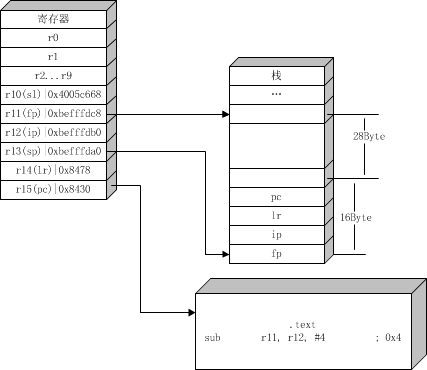
\includegraphics[bb=0 0 427 370,scale=0.7]{armapcs1_6.png}
\caption{存储当前的pc lr ip fp ok 上一个栈顶指针-4个字节就是当前的栈帧}
\label{fig:anna}
\end{figure}

\begin{figure}[htbp]%位置选项
\centering
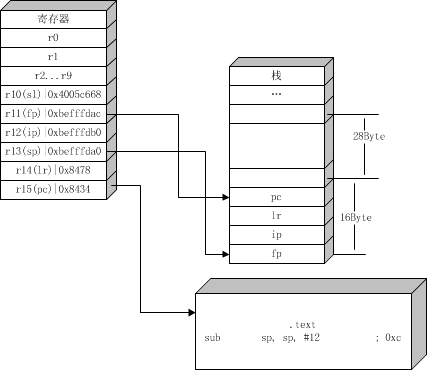
\includegraphics[bb=0 0 427 370,scale=0.7]{armapcs1_7.png}
\caption{当前栈帧计算ok 准备继续在栈上开辟12个字节的空间,方便存储本地自动变量}
\label{fig:anna}
\end{figure}


\begin{code}
存储第一个参数到当前sp之下
0x00008438 <fun1+16>:	str	r0, [r11, #-16]
存储第一个参数到当前sp-4之下
0x0000843c <fun1+20>:	str	r1, [r11, #-20]
存储立即数10到r3寄存器
0x00008440 <fun1+24>:	mov	r3, #10	; 0xa
存储第一个参数到当前sp-8之下
0x00008444 <fun1+28>:	str	r3, [r11, #-24]
存储立即数10到r0寄存器 用于返回值
0x00008448 <fun1+32>:	mov	r0, #0	; 0x0
\end{code}


\begin{figure}[htbp]%位置选项
\centering
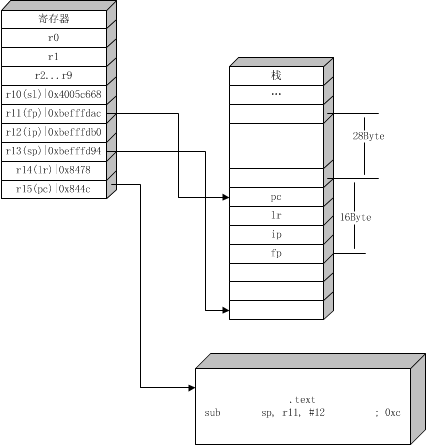
\includegraphics[bb=0 0 427 445,scale=0.7]{armapcs1_11.png}
\caption{当前返回值赋值给r0 ok 准备回退当前栈顶指针到func1栈顶-12处,以便读取内存中已经存储好的lr ip fp 到寄存器的pc sp r11}
\label{fig:anna}
\end{figure}

\begin{figure}[htbp]%位置选项
\centering
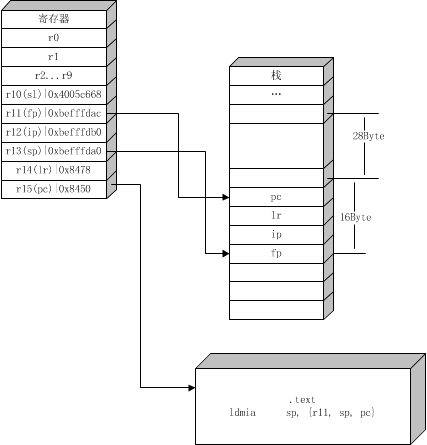
\includegraphics[bb=0 0 427 445,scale=0.7]{armapcs1_12.png}
\caption{回退当前栈顶指针到func1栈顶-12 ok,准备读取内存中已经存储好的lr ip fp 到寄存器的pc sp r11}
\label{fig:anna}
\end{figure}

\begin{figure}[htbp]%位置选项
\centering
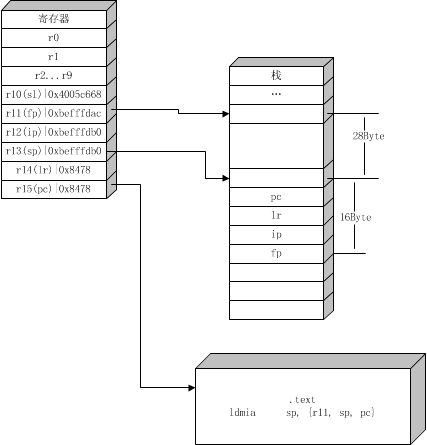
\includegraphics[bb=0 0 427 445,scale=0.7]{armapcs1_13.png}
\caption{读取内存中已经存储好的lr ip fp 到寄存器的pc sp r11 ok 函数回退完毕}
\label{fig:anna}
\end{figure}

%\newpage
